The following chapter is included to show that the developed hybrid diffusion solver can be applied to real life problems with only minor modifications.

\section{Physical scope}

\begin{figure}[H]
 \centering
 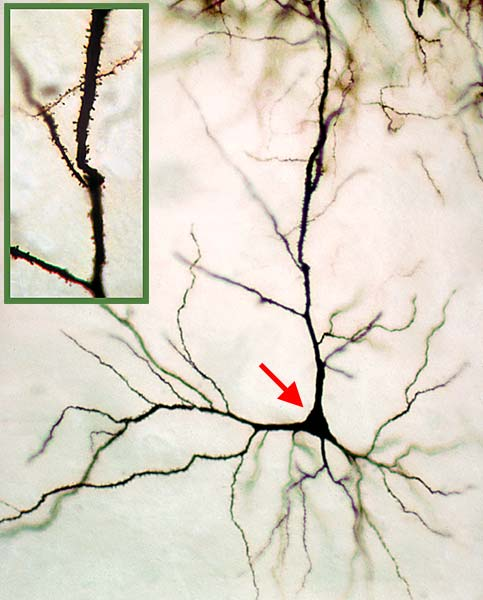
\includegraphics[width=0.7\textwidth]{Figures/Cochlear_nucleus_multipolar_cell.jpg}
 \caption[Pyramidal neuron]{A pyramidal neuron with an apical dendrite (staring by the arrow). The inset shows an amplification of the apical dendrite and illustrates the size of dendritic spines (small outgrowths). The arrow points to the cell body, called the Soma. Note that this image does not show how neurons are located within the brain. Image from \url{www.neurolex.org}.}
 \label{application:pyramidal_neuron}
\end{figure}

Figure \ref{application:pyramidal_neuron} shows a pyramidal neuron with an apical dendrite, and an inset with dendritic spines. 
Spines are (often) the receiving end of a chemical synapse, which is a junction between two neurons. 
This application will look at the diffusion of PKC$\gamma$ in the apical dendrite and into dendritic spines. 
PKC$\gamma$ is a protein found in neurons which is associated with memory storage and associative learning \cite{saito2002protein}. 
Upon activation it will diffuse out of the Soma, through a dendrite, and into a dendritic spine to reinforce or reduce the absorption of neurotransmitters. 
The results will be compared to results by Craske et.al \cite{craske2005spines}, who in 2005 studied a similar problem in rodent pyramidal neurons harvested from the hippocampus.

Effectively we will investigate the diffusion time for random walkers through spine necks which are very narrow ($\leq0.5\mu$m). 

\section{Implementation}

There is a difference between the approach of the developed hybrid solver and the dendrite - spine system with respect to geometry which is best summarized in figure \ref{application:geometry_difference}.\\

\noindent The dendrite is approximated as a cylinder with radius $\sim10\mu$m and length $\sim50\mu$m. Furthermore, little of interest is assumed to happen in the radial direction. All things considered, diffusion in the dendrite will be modeled as a 1D process. \\

\noindent Spines have a wide variety of geometries, with various properties. For this application, however, only the neck length and width of a spine is of interest. The spines will therefore be modeled as two dimensional objects with a funnel shape. 
\begin{figure}[H]
 \centering
 \begin{subfigure}{0.48\textwidth}
  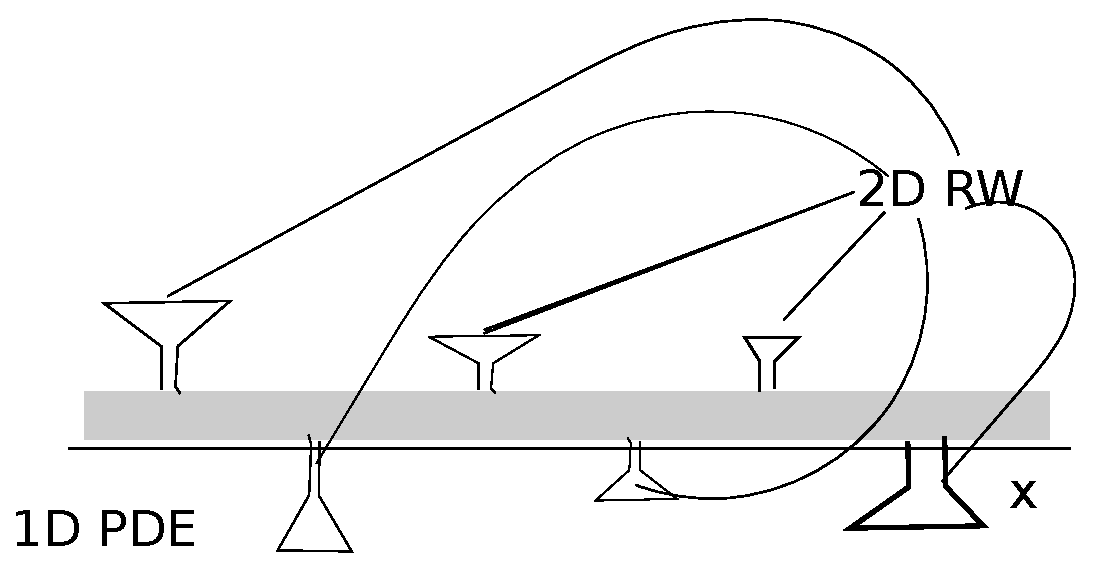
\includegraphics[width=\textwidth]{Figures/dendrite_spine_model.eps}
  \caption{}
 \end{subfigure}
 \begin{subfigure}{0.48\textwidth}
  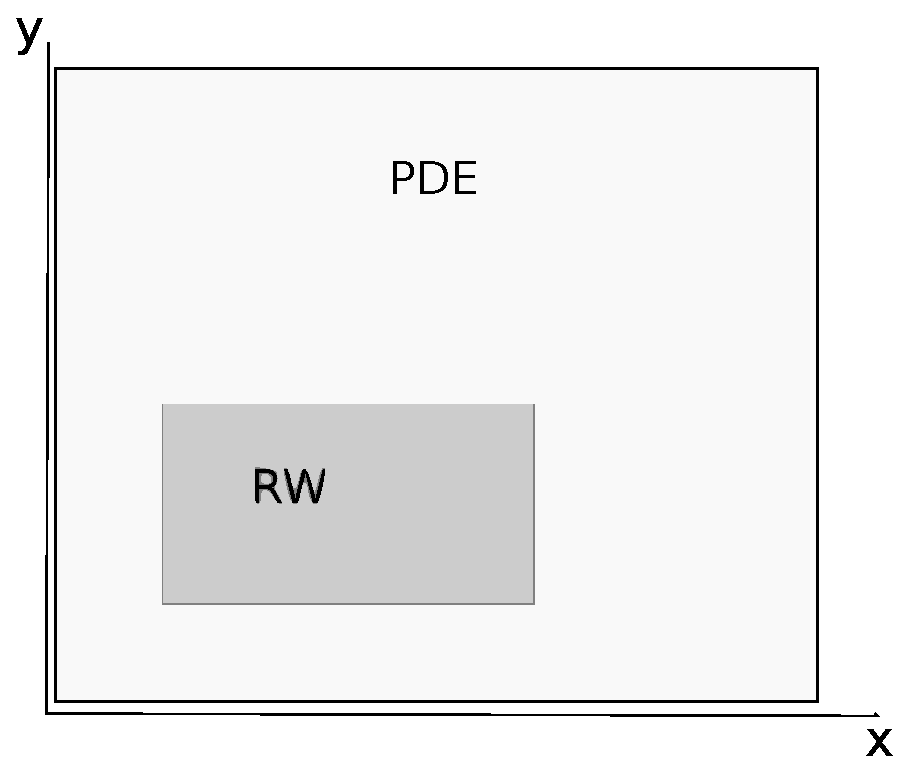
\includegraphics[width=\textwidth]{Figures/hybrid_model_principle.eps}
  \caption{}
 \end{subfigure}
 \caption[Difference between hybrid diffusion solver and dendrite - spine diffusion model]{The geometric difference between the original hybrid diffusion solver (b) and the problem of PKC$\gamma$ diffusing into dendritic spines (a). }
 \label{application:geometry_difference}
\end{figure}

The hybrid diffusion solver has been slightly modified in order to recreate the new geometry. 
Mathematically the largest difference is that the random walkers are left alone, meaning that the diffusion equation is not solved in the spines. 
There are also some differences in the coupling; at each PDE time step there is a probability for an enzyme to diffuse into a spine if the concentration at the beginning of the spine neck is large enough. This probability decreases with the number of enzymes which have already diffused into the spine. 
The width of a spine neck is determined by the number of PDE mesh points it connects to, which is chosen at random. 
All other length parameters are also determined randomly, but required to fit with measurements from Arrelano et.al \cite{arellano2007ultrastructure}. 

\subsection{Initial Condition}

In the presence of glutamate the diffusion constant for PKC$\gamma$ has been measured to $0.33\frac{\mu m^2}{s}$, but this does not reproduce the diffusion times in dendrites which are illustrated by Craske et.al. 
There are two possible fixes to this; \emph{\textcolor{red}{either I have read the paper wrong, and the diffusion constant is really $5.72$ in the dendrite, in which case everything is ok.}} 
The other possibility is to modify the initial condition. The latter is not as far fetched as is sounds because there is considerable absorption of PKC$\gamma$ in the dendrite walls during the first few seconds after release from soma. 
The modified initial condition can be viewed as the concentration distribution in the dendrite some 2 seconds after release from soma.
\clearpage

\section{Parameters}

The new problem requires the introduction of some additional parameters as well as a reformulation of limiting factors for some known parameters, all of which are described in the following table.
 
 \begin{table}[H]
\centering
\begin{tabular}{|p{0.13\textwidth}|p{0.21\textwidth}|p{0.18\textwidth}|p{0.37\textwidth}|}
\hline
\textbf{Parameter} & \textbf{Explanation} &\textbf{Expression/ typical value}& \textbf{Origin} \\
\hline
$\Delta t$ & time-step & $\Delta x^2$ & stability criterion FE scheme \\
\hline
$\Delta x$ & spatial resolution & $\frac{1}{2}$min(spine neck diameter) & estimated \\
\hline
$Hc$ & conversion factor & 5-24 & estimated by calculations of concentration levels taken from \cite{light1996protein} and spine/dendrite volume ratios. See later for discussion. \\
\hline
$u(t=0)$ & initial condition value & 5$\frac{\text{nMol}}{\text{L}}$ & estimated from values found in \cite{light1996protein}\\
\hline
$p_{ds}$ & probability to diffuse into a spine & $0.1\cdot\Delta x\cdot\Delta t$& estimated. An important ability of this parameter should be that wide necked spines have larger probability and that a certain flux is maintained (on average), meaning that the flux should be independent of $\Delta t$ \\
\hline
$p_{ab}$ & probability for PKC$\gamma$ to be absorbed, and removed from simulation, per time-step taken in spine head & 100\% & estimated\\
\hline
\end{tabular}
\caption[Important parameters]{Parameters which play an important role in the simulation of PKC$\gamma$ diffusion into dendritic spines with explanations, expressions/typical values and an indication as to where the value/expression has its origin.}
\label{table:parameters}
\end{table}
